\documentclass[a5paper, 10pt]{book}
\usepackage{ucs}
\usepackage[utf8]{inputenc}
\usepackage[T1]{fontenc}
\usepackage[english,ngerman]{babel}
\usepackage{verbatim}
\usepackage[a5paper]{geometry}
\usepackage{scrextend}
\usepackage{parskip}
\usepackage{url}
\usepackage{graphicx}
\usepackage{xcolor}
\usepackage{titling}
\usepackage{marginnote}
\usepackage[contents={},opacity=1,scale=1,angle=90]{background}
\usepackage{tikz}
\usepackage{tgadventor}
\usepackage{fancyhdr}
\usepackage{setspace}
\usepackage{palatino}
\usepackage{style}

\begin{document}
    %----- document settings ---------------------------------------------------
	%language settings
		\selectlanguage{ngerman}
    %set text alignment
		%default = justified
    %set line height
    	\linespread{1}
	%graphicspath
		\graphicspath{ {./img/} }
	%format page
		\newgeometry{left = 2cm, right = 2cm, marginparwidth = 0cm, marginparsep = 0cm}
	%format numbering
		\pagenumbering{gobble}
	%typographical settings
		\sloppy

    %----- document settings ---------------------------------------------------

	%----- document information ----------------------------------------------------

	\title{GroupMatcher}
	\def \subtitle {Handbuch}
	\author{Justus Roßmeier, Max Obermeier}
	\date{\today}

	%----- document information ----------------------------------------------------
	\BgUsefalse
    %----- title ---------------------------------------------------------------
	\BgFtrue

	\maketitle

	\BgFfalse

	\tableofcontents

    %----- title ---------------------------------------------------------------

    %----- content -------------------------------------------------------------

	\newgeometry{inner = 1.5cm, outer = 4cm, marginparwidth = 2.75cm, marginparsep = 0.75cm}
	\pagenumbering{arabic}
	%select default fonts
		\renewcommand*\rmdefault{qag}
		\fontfamily{ppl}\selectfont
	\BgUsetrue


	\chapter{Einführung}
\label{ch:einführung}

\paragraph{Das Produkt} Das Open-Source Programm >>GroupMatcher<< , dass auf Go \mnote{Go bzw. >>golang<< ist eine 2009 erschienene Programmiersprache, die auf Serverstrukturen spezialisiert ist.} basiert, dient zur Verteilung von Personen auf Gruppen unter Berücksichtigung ihrer Wünsche. Dabei können die Personen, die über Erst-, Zweit- und Drittwunsch verfügen, auf eine beliebige Anzahl von Gruppen mit nach oben und unten begrenzbarer Mitgliederzahl verteilt werden. Diese Aufgabe übernimmt ein Verteilungsalgorithmus, der stets erstklassige Ergebnisse erzielt. Trotzdem bietet die Benutzeroberfläche nützliche Werkzeuge, die manuelle Nachverteilungen erheblich erleichtern.
\paragraph{Die Entwicklung} Die Anwendung wurde im Rahmen eines Informatikkurses in der elften Jahrgangsstufe eines bayerischen Gymnasiums von Justus Roßmeier und Max Obermeier entwickelt. Vielen Dank gehen dabei auch an den Initiator des Projekts, Christian Hoffelner, für die Unterstützung und Betreuung der Arbeit.

	\chapter{Installation}
\label{ch:installation}

Der >>GroupMatcher<< ist eine portable Software \mnote{Portable Software muss nicht installiert werden und kann deshalb auch auf externen Datenträgern mitgeführt werden.}. Während sie auf den Betriebssystemen \hl{Linux} und \hl{MacOS} lediglich die Anwendungsdatei ausführen müssen, um das Programm in ihrer Systemsprache zu starten, ist es auf \hl{Microsoft Windows} zu empfehlen, eine der im Programmverzeichnis enthaltenen Verknüpfungen zu verwenden. Diese sind mit Landeskennungen \mnote{z.B.: >>DE<< oder >>EN<< } versehen, welche sich auf die Sprache der Benutzerfläche beziehen. Die Verknüpfung >>GroupMatcherDE<< wird das Programm in der Ausgangssprache >>Deutsch<< starten. Auch wenn die Sprache des Programms noch während der Laufzeit angepasst werden kann, wie in \ref{sec:menüleiste} erläutert wird, ist so eine zeitsparendere Alternative geboten.

	\chapter{Benutzeroberfläche}
\label{ch:benutzeroberfläche}

\begin{figure}
	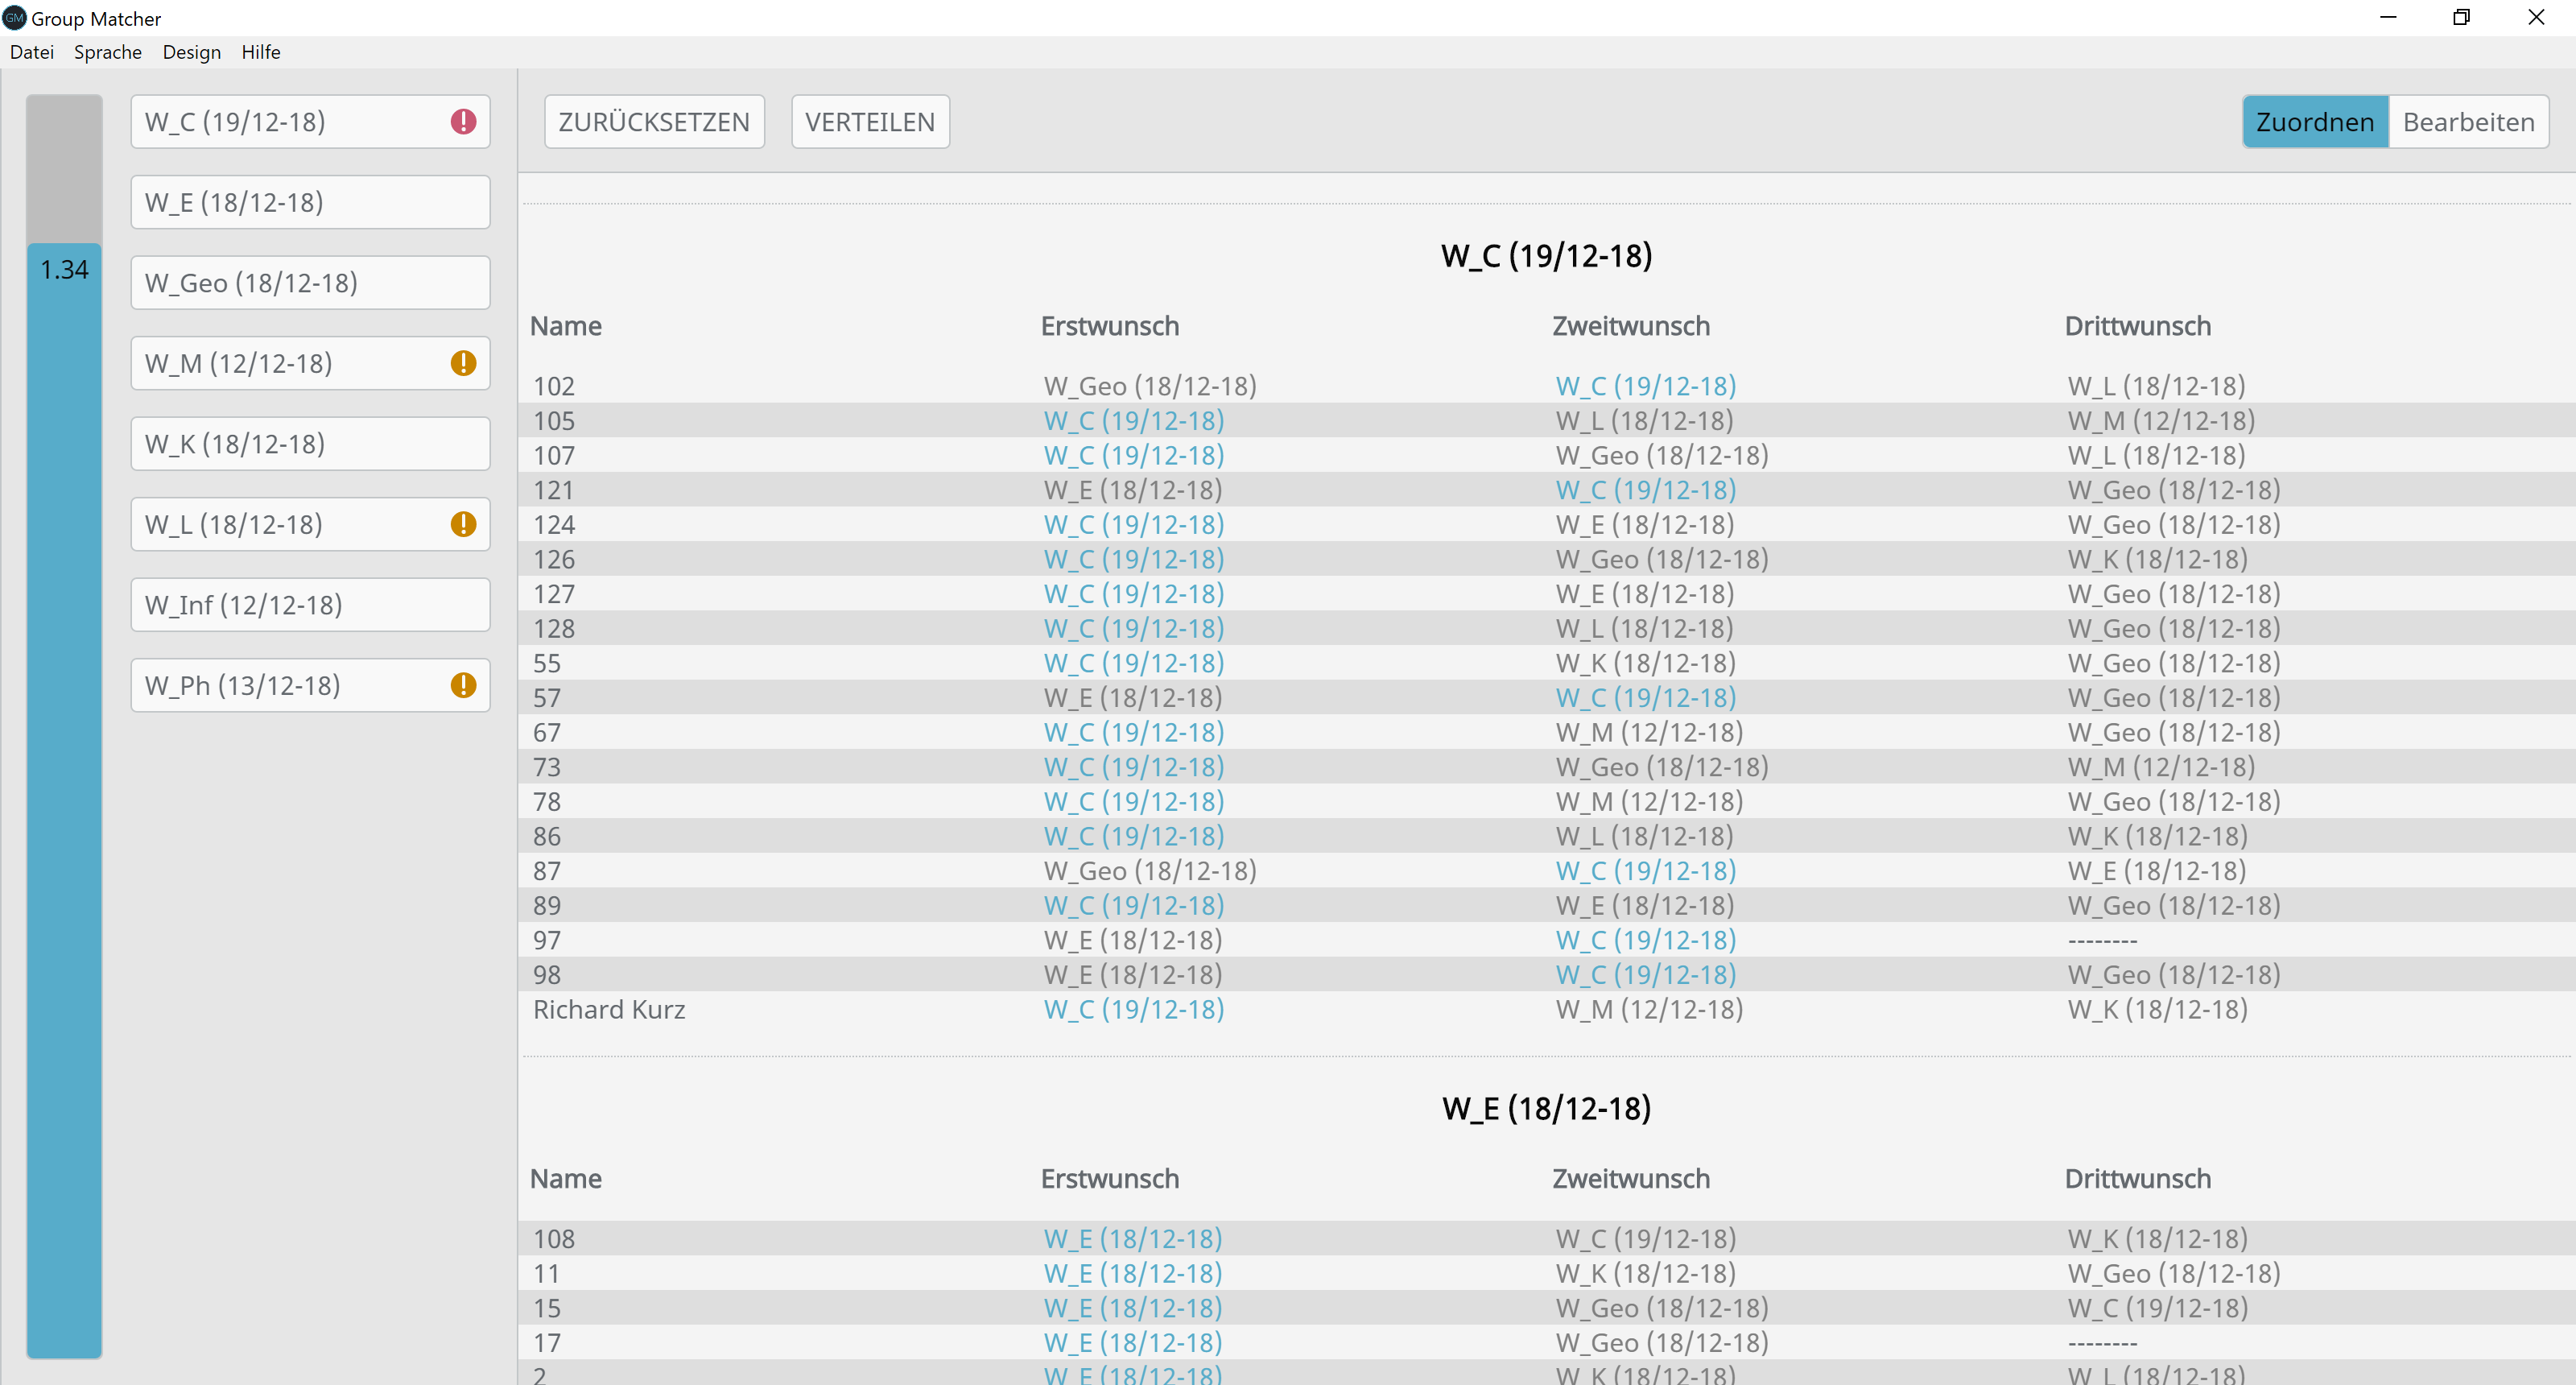
\includegraphics{zuordnungsmodus}
	\caption{Die Benutzeroberfläche}
	\label{fig:die_benutzeroberfläche}
\end{figure}

Die Benutzeroberfläche, die in Abbildung \ref{fig:die_benutzeroberfläche} dargestellt ist, besteht aus vier Bereichen:
\begin{itemize}
	\item Die \hl{Menüleiste}(\ref{sec:menüleiste}) befindet sich in voller Breite ganz oben im Fenster.
	\item Die \hl{Seitenleiste}(\ref{sec:seitenleiste}) nimmt den linken Rand des Bildschirms ein.
	\item Die \hl{Bedienzeile}(\ref{sec:bedienzeile}) ist links von der Seitenleiste und oben von der Menüleiste begrenzt.
	\item Die \hl{Arbeitsfläche}(\ref{sec:arbeitsfläche}) nimmt den Rest des Fensters ein.
\end{itemize}
Die Bedienelemente und deren Nutzen wird im Folgenden erläutert.

\section{Menüleiste}
\label{sec:menüleiste}

Die Menüleiste dient zur Kontrolle von Programm und Projekt. Sie enthält vier Unterpunkte.

\paragraph{Datei} Hier ist zunächst die Kontrolle des Projekts, also der >>.gm<< Datei \mnote{Im Dateiformat >>.gm<< speichert der >>GroupMatcher<< zum einen die Projekte ab. Zum anderen dient das Format auch zur schnellen Erstellung eines Projekts. Die Syntax dafür wird in Kapitel \ref{TODO: label einfügen} beschrieben.} möglich.
\begin{itemize}
	\item \hl{Öffnen...} (öffnet einen Dialog, der das einlesen eines Projekts, also einer >>.gm<< Datei ermöglicht)
	\item \hl{Schließen} (schließt das Projekt, ohne den aktuellen Zustand zu speichern)
	\item \hl{Speichern} (speichert den aktuellen Stand in die geöffnete >>.gm<< Datei)
	\item \hl{Speichern unter...} (öffnet einen Dialog, der das Speichern des aktuellen Standes in eine neue >>.gm<< Datei ermöglicht, und schließt (sofern vorhanden) die alte >>.gm<< Datei)
	\item \hl{Exportieren...} (öffnet einen Dialog, der das erstellen einer Excel-Datei, welche das Projekt darstellt, ermöglicht)
	\paragraph{Excel (begrenzt)} Die begrenzte Version enthält lediglich die Liste der Personen in alphabetischer Reihenfolge mit dem jeweils zugeordneten Wunsch.
	\paragraph{Excel (komplett)} Die komplette Version gibt alle Projektinformationen wieder. Sie listet alle Gruppen mit minimaler und maximaler Mitgliederzahl, sowie der nach der Zuteilung tatsächlich entstandenen Gruppenstärke auf. Zudem stellt sie jede Person mit ihren Wünschen dar und hebt dabei den ihr zugeteilten farblich hervor.
	\item \hl{Beenden} (schließt das Programm und speichert, insofern schon eine >>.gm<< Datei erstellt wurde, das Projekt in diese ab)
\end{itemize}

\paragraph{Sprache} Dieses Untermenü ermöglicht das Wechseln zwischen den bereitgestellten Sprachen.

\paragraph{Design} Neben den hellen Standarddesign lässt sich bei dunkler Umgebung auf das für die Augen angenehmere dunkle Design umschalten.

\paragraph{Hilfe} Neben dem öffnen dieser Dokumentation im Punkt >>Hilfe<< können hier im Punkt >>Über GroupMatcher<< weitere Informationen über Ursprung, aktuelle Versionen und Lizensierung des Programms gewonnen werden.

\section{Seitenleiste}
\label{sec:seitenleiste}

Die Seitenleiste gibt eine Übersicht über das Projekt und erleichtert die Navigation in der Arbeitsfläche. Die blaue Skala zeigt die aktuelle Quote \mnote{Die Quote gibt an, wie zufrieden die Personen durchschnittlich mit ihrer Zuteilung sind. Die genaue Berechnung wird in Abschnitt \ref{TODO:referenz einfügen} genauer erläutert. Generell gilt aber, je höher der blaue Balken, desto besser das Ergebnis.}.\\
Rechts daneben sind alle Gruppen aufgelistet. Dabei wird erst der Gruppenname und dann in Klammern zunächst die aktuelle Gruppenstärke, dann die Mindest- und Maximalgröße der Gruppe angezeigt. Drückt man auf den Knopf einer Gruppe, so scrollt die Arbeitsfläche zu deren Position. Die Knöpfe können zwei verschiedene Warnungen anzeigen. Erscheint ein orangenes Ausrufezeichen, dann bedeutet dies, dass die Gruppe ein Mitglied hat, das unzufrieden \mnote{Unzufriedenheit bedeutet dabei, dass der Person ein Wunsch zugeordnet wurde, der in der hinteren Hälfte seiner Wunschliste steht.} mit seiner Zuteilung ist. Leuchtet stattdessen ein rotes Ausrufezeichen auf, so widerspricht die aktuelle Gruppenstärke der Mindest- oder Maximalgröße der Gruppe. Dieser Fall tritt jedoch nie durch die automatische Verteilung auf, sondern kann nur in der manuellen Nachverteilung herbeigeführt werden. Mehr zum Verteilungsvorgang finden sie in Kapitel \ref{ch:verteilen_der_personen}.

	\chapter{Erstellen eines Projekts}
\label{ch:erstellen_eines_projekts}

Liegt noch kein Projekt in Form einer >>.gm<< Datei vor, so muss dies erst erstellt werden. Dazu starten sie das Programm wie es in Kapitel \ref{ch:installation} erklärt wurde. Nun wechseln sie in den Bearbeitungsmodus. Sie sehen in der Arbeitsfläche ein leeres Textfeld. Dort müssen sie nun ihre Gruppen und Personen in der >>.gm<< Syntax eintragen, was im Folgenden Abschnitt erklärt wird.

\section{>>.gm<< Syntax}
\label{sec:>>.gm<<_syntax}

Hier wird erklärt, wie eine >>.gm<< Datei aufgebaut ist. In der folgenden Weise werden nicht nur >>GroupMatcher<< Projekte gespeichert, sondern auch vom Benutzer erstellt. Dank dem einfachen Aufbau ist die Syntax schnell erlernt und dann ist sie wesentlich effektiver als jede graphische Lösung der Bearbeitung. Um die folgende Erläuterung besser zu verstehen, kann zum einen Abbildung \ref{fig:die_syntax} mit der theoretischen Syntax \mnote{In der theoretischen Syntax gelten Folgende Regeln:\\
	- in spitze Klammern (<>) eingeschlossene Wörter stellen Variablen dar\\
	- in eckige Klammern ([]) eingeschlossene Gefüge sind optional\\
	- drei Punkte (...) stehen für eine unbegrenzte Wiederholung des davor stehenden Gefüges
} und zum anderen Abbildung \ref{fig:ein_beispiel} mit einem Beispielcode helfen.

\begin{figure}
	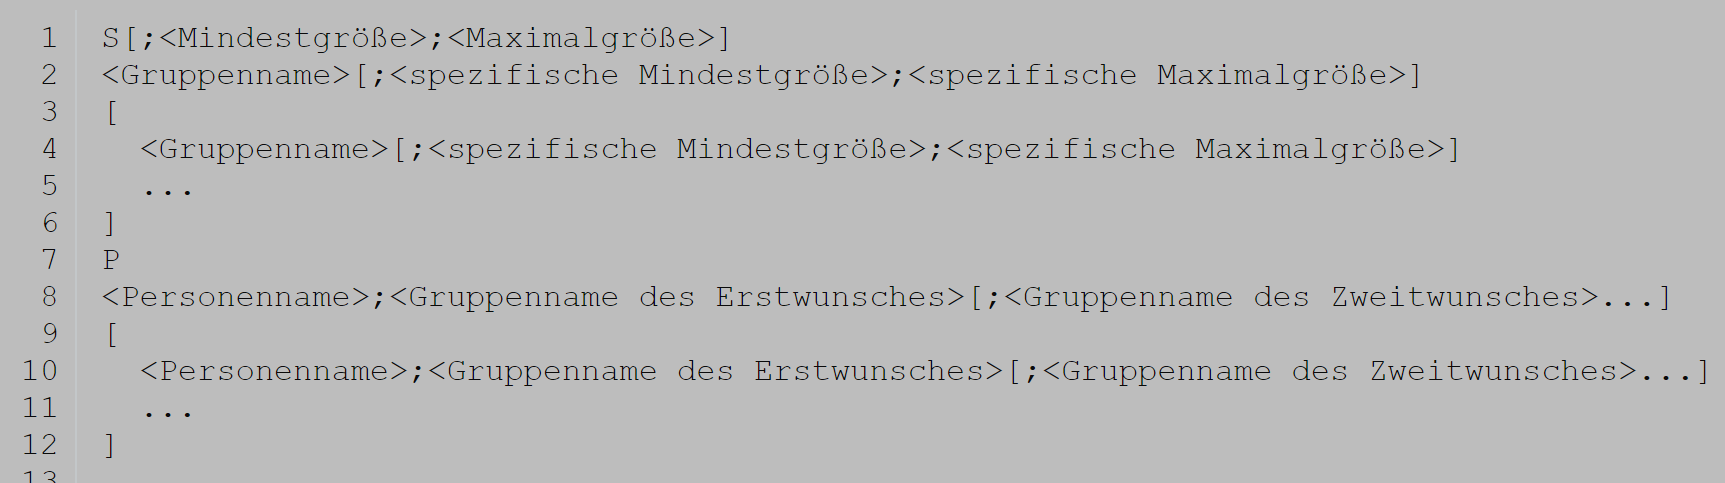
\includegraphics{syntax}
	\caption{Die Syntax der >>.gm<< Dateien}
	\label{fig:die_syntax}
\end{figure}

\begin{figure}
	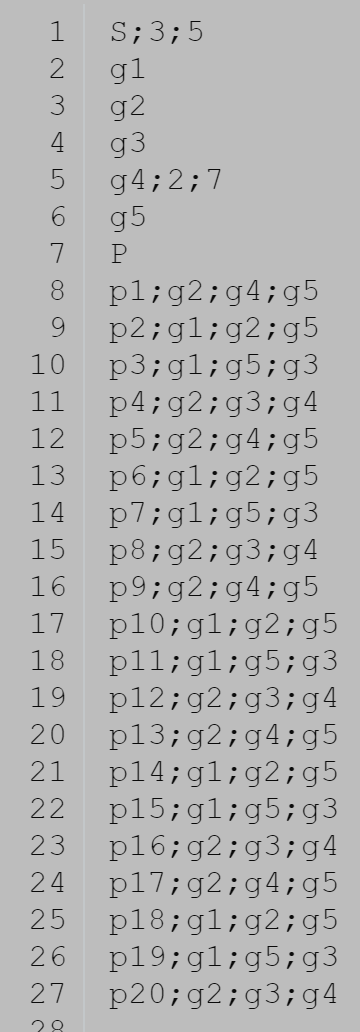
\includegraphics[width=3cm]{beispiel}
	\caption{Ein Beispiel einer >>.gm<< Datei}
	\label{fig:ein_beispiel}
\end{figure}

\paragraph{Gruppendeklaration} Am Anfang der Datei steht der \hl{Gruppenindikator} >>S<<. Dieser zeigt dem Übersetzerprogramm an, dass nun die Informationen für Gruppen folgen. In der Zeile des Gruppenindikators können durch Semikolons \mnote{Semikolon = ;} getrennt eine \hl{allgemeine Mindest- und Maximalgröße} festgelegt werden. Diese gilt dann für alle Gruppen, für die nicht später eigenen Werte festgelegt werden. Wird kein allgemeiner Wert festgelegt, so wird für beide Werte der Wert 0 angenommen.\\
Ab der darauffolgenden Zeile können Gruppen definiert werden. Dabei steht immer am Anfang der Zeile der \hl{Gruppenname}. Soll für die Gruppen nicht die allgemein definierten Werte für Mindest- und Maximalgröße gelten, so können wiederum durch Semikolons getrennt die \hl{spezielle Mindest- und Maximalgröße} festgelegt werden. In jeder Zeile darf dabei immer nur eine Gruppe stehen.
\paragraph{Personendeklaration} Sind alle Gruppen definiert, so folgt in der nächsten Zeile der \hl{Personenindikator} >>P<<.\\
Ab der nächsten Zeile können Personen definiert werden. Dabei steht am Anfang jeder Zeile der \hl{Personenname}, gefolgt von einem Semikolon. Danach kann, durch Semikolons separiert, eine unbegrenzte Anzahl \mnote{Auch wenn im Zuordnungsmodus der Benutzeroberfläche nur drei Wünsche angezeigt werden, unterstützt das Programm bei allen anderen Funktionen eine unbegrenzte Anzahl an Wünschen.}, aber mindestens ein Wunsch festgelegt werden. Dies geschieht durch das Nennen des \hl{Gruppennamens} der gewünschten Gruppe. Sind alle Wünsche festgelegt, so kann die Person einer seiner Wünsche zugeordnet werden, was aber für den Benutzer irrelevant ist, sondern nur beim Speichern des Projekts eine Rolle spielt, was aber vom Programm erledigt wird. Die Syntax dazu ist aber ein Schrägstrich gefolgt von dem Gruppennamen des erfüllten Wunsches. Pro Zeile darf wiederum nur eine Person deklariert werden.

\section{Abschließen des Erstellvorgangs}
\label{sec:abschliessen_des_erstellvorgangs}

Wurden alle Gruppen und Personen wie oben erklärt erstellt, so kann nun mit der Zuteilung begonnen werden. Dazu betätigen \mnote{Drücken sie auf zuordnen.} sie den Wechselschalter in der oberen rechten Ecke. Falls nun eine Fehlermeldung erscheint versuchen sie diese zu beheben. Dabei kann ihnen das Kapitel \ref{ch:fehlermeldungen} helfen. Ansonsten gelangen sie jetzt in den Zuordnungsmodus. Zugleich öffnet sich ein Dialog, der sie zum speichern des Projekts auffordert. Dies sollten sie nun unbedingt tun, da das Projekt verfällt, falls noch kein Speicherpfad angegeben ist, wenn das Programm geschlossen wird. Haben sie das Projekt erfolgreich gespeichert, so ist der Erstellvorgang abgeschlossen.

	\chapter{Verteilen der Personen}
\label{ch:verteilen_der_personen}

Im Verteilungsverfahren liegt die größte Stärke des >>GroupMatcher<<. Haben sie nämlich das Projekt erstellt, so müssen sie nur im Zuordnungsmodus auf den Knopf >>verteilen<< \mnote{Den Knopf finden sie in der Bedienzeile.} klicken und der Algorithmus des Programms verteilt die Personen auf die Gruppen. Danach können sie eine manuelle Nachverteilung vornehmen, falls spezielle Wünsche vorliegen. Sie müssen sich keine Gedanken um die Gerechtigkeit des Algorithmus machen, da dieser nach dem Zufallsprinzip arbeitet. Die Reihenfolge, in der sie die Personen in der >>.gm<< Datei definieren spielt also keine Rolle.

\section{Verteilungsalgorithmus}
\label{sec:verteilungsalgorithmus}

\paragraph{Prioritäten} Der Verteilungsalgorithmus arbeitet nach folgenden Prioritäten:
\begin{enumerate}
	\item jede Person muss einer Gruppe zugeordnet werden
	\item keine Person darf einer Gruppe zugeordnet werden, die nicht in seinen Wünschen enthalten ist
	\item Gruppen dürfen nur entfernt werden, wenn nicht genügend Personen existieren, in deren Wünschen die Gruppe enthalten ist, um die Minimalgröße zu erfüllen
	\item die Minimal- und Maximalgröße einer Gruppe darf nicht über- bzw. unterschritten werden
	\item die Quote \mnote{Die Quote stellt den durchschnittlich erfüllten Wunsch dar. Wurden nur Erstwünsche erfüllt, so ist die Quote also 1. Wurden zur Hälfte Erstwünsche und zur anderen Hälfte Zweitwünsche erfüllt, so beträgt die Quote 1.5. } soll bestmöglich sein
\end{enumerate}

\paragraph{Wegfallen einer Gruppe} Sind für eine Gruppe zu wenige Wünsche vorhanden, so wird diese und die entsprechenden Wünsche gelöscht. Darf dies nicht auftreten, so muss speziell für diese Gruppe die Mindestgröße angepasst werden, wie es in Abschnitt \ref{sec:>>.gm<<_syntax} erläutert wird. Soll dies rückgängig gemacht werden, so müssen sie zum vorherigen Speicherstand zurückkehren. Dazu wählen sie >>Datei<< und >>Schließen<< und wählen dann über >>Datei<< und >>Speichern unter...<< die nach dem Erstellen angelegte >>.gm<< Datei aus. Nun können sie, vor dem erneuten ausführen des Verteilungsalgorithmus, eine spezielle Mindest- und Maximalgröße für die betroffene Gruppe festlegen.

\section{Nachverteilung}
\label{sec:nachverteilung}

Wollen sie, aus welchem Grund auch immer, im nachhinein eine Änderung vornehmen, so muss dies nach dem Betätigen des Verteilungsalgorithmus geschehen, da dieser keine bereits zugewiesenen Personen akzeptiert. Die verfügbaren Werkzeuge zum Umverteilen werden in den Abschnitten \ref{sec:seitenleiste} und \ref{sec:arbeitsfläche} erklärt. Sind sie mit der Verteilung zufrieden sollten die das Projekt wiederum abspeichern \mnote{>>Datei<< und >>Speichern<<}.

	\chapter{Abschließen eines Projekts}
\label{ch:abschliessen_eines_projekts}

	\chapter{Fehlermeldungen}
\label{ch:fehlermeldungen}

\paragraph{>>Verteilen nicht möglich: Zu viele oder zu wenige Personen für gewählte Gruppenkonfiguration<<} Die Gesamtanzahl der Personen ist zu groß oder zu klein für die Gruppengrößen.

\paragraph{>>Übersetzungsfehler:<<} Alle Fehlermeldungen, beziehen sich auf den Übersetzungsvorgang der >>.gm<< Datei.

\paragraph{>>Syntaxfehler<<} Die >>.gm<< Syntax wurde nicht eingehalten.

\paragraph{>>Indikator für Gruppen nicht gefunden<<} Das >>S<<, der Indikator für die Gruppen wurde nicht gefunden.

\paragraph{>>mehrfache Benutzung eines Gruppennamens<<} Jede Gruppe muss einen einzigartigen Namen haben. Achten sie dabei auch auf den Personenindikator >>P<<, der nicht alleinstehend als Gruppenname benutzt werden darf.

\paragraph{>>mehrfache Benutzung eines Personennamens<<} Jede Person muss einen einzigartigen Namen haben.

\paragraph{>>leere Datei<<} Die importierte Datei ist leer.

\paragraph{>>Indikator für Personen nicht gefunden<<} Der Personenindikator >>P<< sollte direkt unter der Gruppenauflistung stehen.

\paragraph{>>leeres Argument<<} Hinter einem Semikolon muss immer ein Inhalt sein. Wenn sie einer Person z.B. nur zwei Wünsche zuordnen wollen, darf diese Zeile auch nur zwei Semikolons enthalten.

\paragraph{>>fehlendes Argument<<} Jede Person muss mindestens einen Wunsch haben. Die Gruppenstärken müssen entweder allgemein hinter dem Gruppenindikator, oder speziell für jede einzelne Gruppen bei der Gruppenaufzählung festgelegt werden.

\paragraph{>>eine Gruppe ist nicht vorhanden<<} Alle Gruppen, die in Wünschen auftauchen, müssen vorher in der Gruppenauflistung definiert werden.

\paragraph{>>eine Person konnte nicht zugeteilt werden<<} Dieser Fehler kann auftreten, wenn bei einer Person alle Wünsche ungültig sind, weil die entsprechenden Gruppen aufgrund von Unterbesetzung entfernt wurden.

\paragraph{>>Folgende Gruppe(n) kam(en) nicht zusammen:<<} Ist eine Gruppe unterbesetzt, d.h. kann die Mindestgröße nicht erreicht werden, wird sie automatisch gelöscht, und entsprechende Wünsche entfernt. Danach wird versucht, ohne diese Gruppe eine Verteilung zu finden.

\paragraph{>>Sprache nicht gefunden<<} Dieser Fehler kann nur auftreten, wenn in der URL, oder im Programmverzeichnis manuelle Änderungen vorgenommen wurden.

\paragraph{>>Keine Gruppen vorhanden<<} Tritt auf, wenn beim Exportieren, oder beim Wechseln in den Bearbeitungsmodus keine Gruppen vorhanden sind.

\paragraph{>>Es sind bereits Personen zugeteilt<<} Der automatische Verteilungsvorgang kann nur gestartet werden, wenn alle Personen unzugeordnet sind.

\paragraph{>>Gruppenkombination(en) überfüllt:<<} Es werden alle Gruppenkombinationen aufgelistet, die überfüllt sind. Dies tritt auf, wenn z.B. die Gruppen x,y eine Maximalgröße von je zwei Personen haben, aber fünf Personen nur die Wünsche x und y haben.

\paragraph{>>Zeitüberschreitung - keine Lösung gefunden<<} Dieser Fehler tritt auf, wenn der Verteilungsprozess nach einer Minute immer noch keine Lösung gefunden hat. Dies passiert in der Regel nur dann, wenn eine komplexe Form eine Gruppenkombinationsfehlers vorliegt, die vom Algorithmus nicht erfasst wird, und keine Lösung möglich ist.

\paragraph{>>Zeitüberschreitung - Lösung gefunden<<} Dieser Fehler tritt auf, wenn der Verteilungsprozess nach zehn Sekunden noch nicht für alle Versuche Lösungen gefunden wurden. Dies tritt v.a. dann auf, wenn die Gruppengrößen sehr eng gewählt wurden, und somit nur sehr wenige Lösungsmöglichkeiten vorhanden sind.






    %----- content -------------------------------------------------------------

\end{document}
